\documentclass[12pt,a4paper,openright]{mwrep}

\usepackage{lmodern}
\usepackage[T1]{polski}
\usepackage[utf8]{inputenc}

\usepackage[a4paper,
            tmargin=2cm,
            bmargin=2cm,
            lmargin=2cm,
            rmargin=2cm,
            bindingoffset=0cm]{geometry}

\usepackage{tocloft}
\usepackage{hyperref}

\usepackage{amsmath}
\usepackage{amssymb}
\usepackage{siunitx}

\usepackage{listings}

\usepackage{graphicx}
\usepackage{subfig}
\usepackage{float}
\usepackage{booktabs}

\hypersetup{
    colorlinks,
    citecolor=black,
    filecolor=black,
    linkcolor=black,
    urlcolor=black
}

\newtheorem{definition}{Def}

\begin{document}

\title{%
Technika cyfrowa\\
Sprawozdanie 1\\
}

\author{\\Jan Chyczyński\\Błażej Nowicki
\\Bartłomiej Słupik\\Przemysław Węglik}

\date{\today}

\maketitle

\chapter{Zadanie 1a}
Zadanie polega na zaprojektowaniu układu realizującego 
funkcję logiczną:
\begin{align*}
    Y = \overline{A}C + B(A + B)
\end{align*}

\section{Rozwiązanie teoretyczne}
Układ można zrealizować wyłącznie dzięki użyciu bramek NAND
ponieważ bramka NAND jest systemem funkcjonalnie pełnym tzn.
korzystając wyłącznie z niej można przedstawić dowolną funkcję
boolowską.

Pierwszym krokiem jest przekształcenie wyrażenie do zawierającego
wyłączenie operacje NAND.
\begin{align*}
    Y &= \overline{A}C + B(A + B) \\
    &= \overline{A}C + B \\
    &= \overline{\overline{\overline{A}C}\overline{B}}
\end{align*}

\section{Symulacja w programie Multisim}
Układ zbudowano w dwóch wersjach: pierwszej, z ręcznymi przełącznikami 
pozwalającymi na zmianę stanu A, B i C oraz drugiej, z generatorem słów bitowych
i analizatorem stanów logicznych.

\begin{figure}[H]
    \centering
    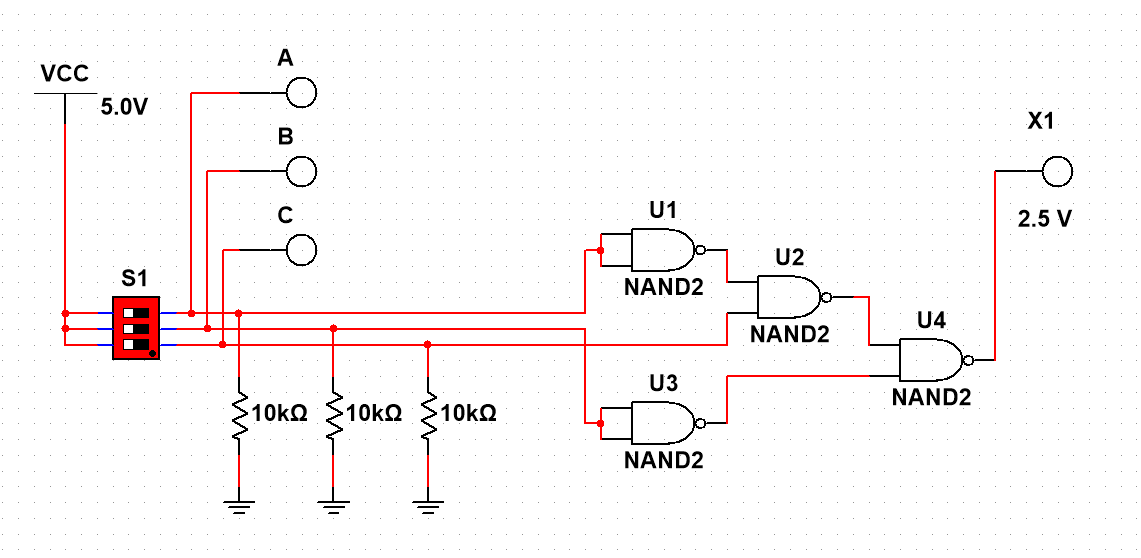
\includegraphics[width=1\textwidth]{images/1a_circuit_simple.png}
    \caption{Układ z ręcznymi przełącznikami}
    \label{rys:1a_circuit_simple}
\end{figure}

\begin{figure}[H]
    \centering
    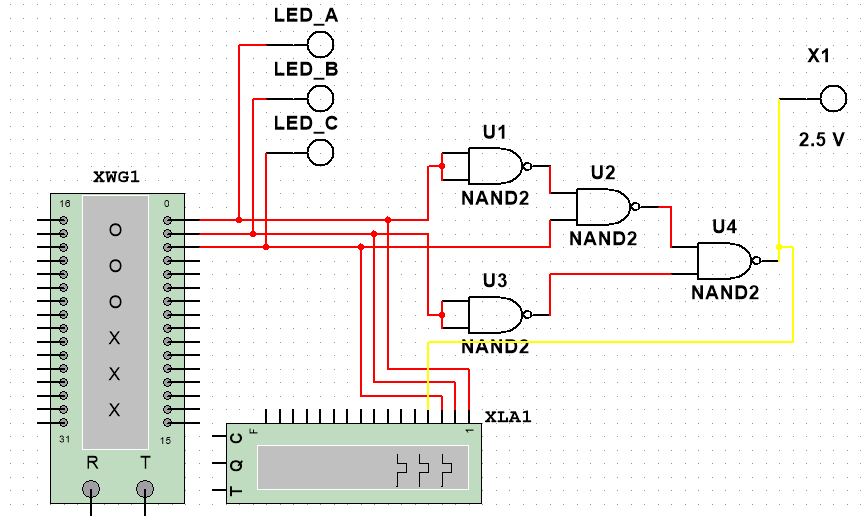
\includegraphics[width=1\textwidth]{images/1a_circuit_word_generator.png}
    \caption{Układ z generatorem i analizatorem}
    \label{rys:1a_circuit_with_generators}
\end{figure}

\begin{figure}[H]
    \centering
    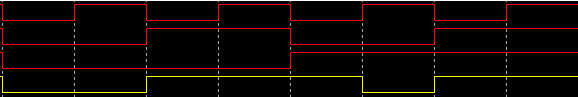
\includegraphics[width=0.8\textwidth]{images/1a_timeseries.png}
    \caption{Przebieg czasowy sygnałów. Od góry: A, B, C, Y}
    \label{rys:1a_timeseries}
\end{figure}

\newpage
\section{Wnioski}
\begin{enumerate}
    \item Dzięki prawom logiki możemy uprosić skomplikowane wyrażenia
    w taki sposób, aby używały mniejszej ilości operacji logicznych.
    \item Przedstawienie funkcji logicznej tylko za pomocą bramek NAND
    ma praktyczne zastosowanie, ponieważ komercyjnie dostępne chipy często
    zawierają kilka bramek tego samego rodzaju (np. 4xNAND, 4xOR itp.).
    Dzięki uproszczeniu układu do bramek NAND, możemy go skonstruować
    w rzeczywistością używając tylko jednego chipu 4xNAND zamiast
    trzech różnych: 4xNOT, 4xOR i 4xAND.
    \item Podana funkcja logiczna po drobnym przekształceniu
    \begin{align*}
        Y = \overline{A}C + B(A + B) = \overline{A}C + B
    \end{align*}
    przedstawia równanie charakterystyczne przerzutnika 
    asynchronicznego typu RS. 
    Po podstawieniach
    \begin{align*}
        A &= R\\
        B &= S\\
        C &= Q_{n-1}\\
        Y &= Q_{n}\\
    \end{align*}
        
    otrzymujemy
    \begin{align*}
        Q_{n} = S + \overline{R}Q_{n-1}
    \end{align*}
\end{enumerate}
\chapter{Zadanie 1b}
Celem zadania jest zaprojektowanie, zbudowanie i przetestowanie 
układu detekcji liczby pierwszej w binarnym słowie czterobitowym.
\section{Rozwiązanie teoretyczne}
W binarnym czterobitowym słowie można zapisać liczby od 0 do 15.
Liczby pierwsze w tym zakresie to 2,3,5,7,11,13.
Przy oznaczeniach wartości bitów A,B,C,D w kolejności od najbardziej znaczącego funkcja logiczna ma postać
\begin{align*}
    f(A,B,C,D) = \sum(2,3,5,7,11,13)
\end{align*}
W celu wyznaczenie najprostszej postaci wpisano ją w tabeli Karnough
    
\begin{table}[h!]
    \centering
    \begin{tabular}{|c|cccc|}
        \hline
        AB/CD & 00 & 01 & 11 & 10 \\
        \hline
        00 & 0 & 0 & 1 & 1 \\
        01 & 0 & 1 & 1 & 0 \\
        11 & 0 & 1 & 0 & 0 \\
        10 & 0 & 0 & 1 & 0 \\
        \hline
    \end{tabular}
    \caption{Tabela Karnough dla badanej funkcji}
\end{table}
Z tabeli można odczytać postać funkcji logicznej
\begin{align*}
    f(A,B,C,D) = B\bar{C}D  + \bar{A}CD 
    + \bar{A}\bar{B}C + C\bar{B}D   \\ 
\end{align*}
Stosując prawa przekształceń równoważnych
\begin{align*}
    f(A,B,C,D) &= B\bar{C}D 
    + \bar{A}\bar{B}C + CD(\bar{A} + \bar{B})   \\ 
    f(A,B,C,D) &= \overline{(A + B)}C + B\bar{C}D 
    +  CD\overline{(AB)}\\
\end{align*}
\section{Budowa i symulacja układu w programie mulitsim}
W celu konstrukcji układu należy przełożyć wzór funkcji na bramki logiczne.
Funkcja jest alternatywą trzech składników.
Pierwszy z nich $ \overline{(A+B)} C $ można reprezentować
przez bramkę NAND i AND. Wyrażenie $ B\bar{C}D $ można zastąpić bramką NOT i AND3
a $ CD\overline{(AB)} $ jako połączenie NOR i AND.
Trzy wyrażenia połączone zostały bramką logiczną OR3. 
Słowa bitowe reprezentujące testowane liczby można wprowadzać przez cztery przełączniki.
Gdy wprowadzone zostanie słowo reprezentujące liczbę pierwszą zapala się dioda.

Opisany schemat w programie multisim.
\begin{figure}[H]
    \centering
    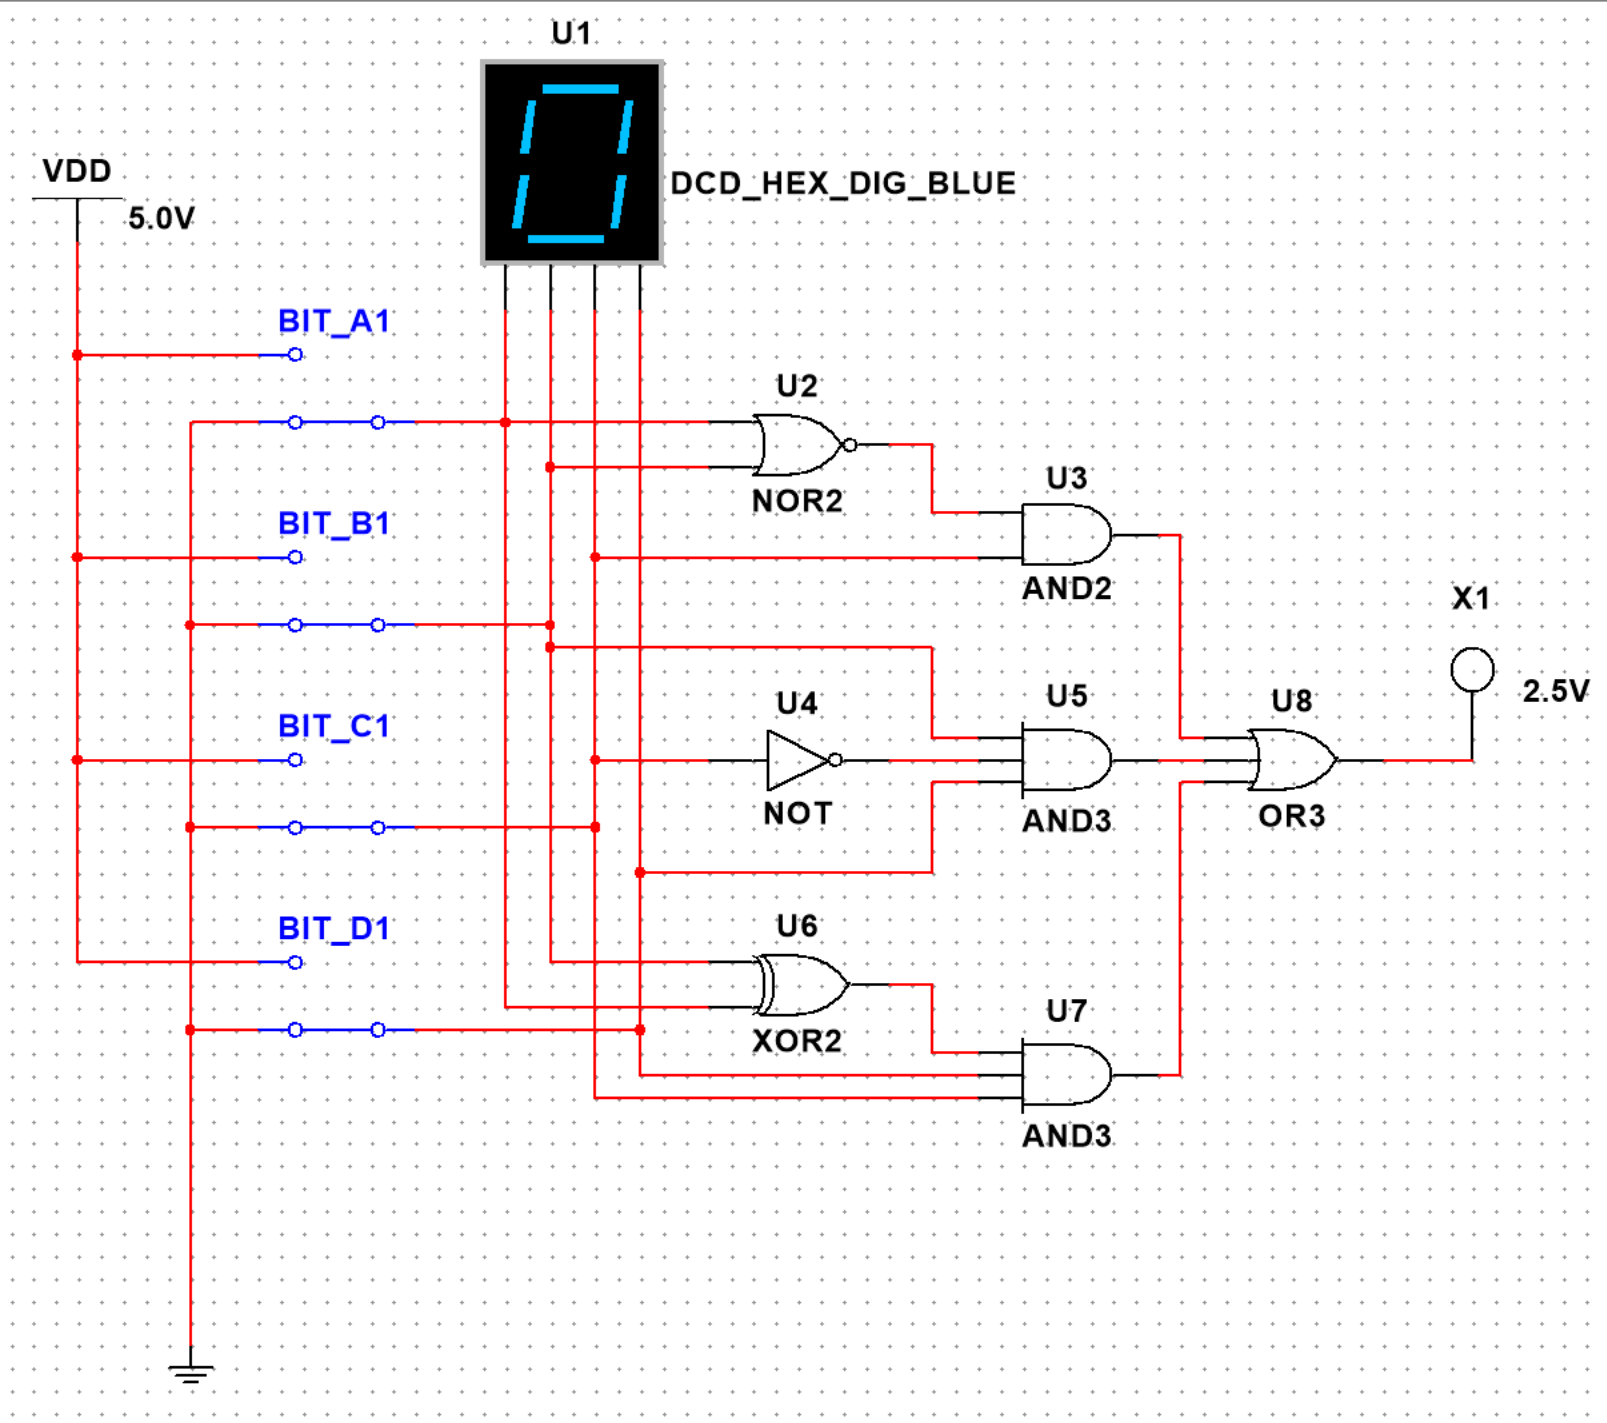
\includegraphics[width=1\textwidth]{images/1b_schema_1.PNG}
    \caption{Układ z ręcznymi przełącznikami}
    \label{rys:1b_usable_circuit}
\end{figure}

W celu kompleksowego przetestowania układu przyciski zamieniono na generator słów bitowych XWG1 
oraz podłączono analizator stanów logicznych XLA1.
Odpowiednio dobierając częstotliwości próbkowania i generowanych sygnałów możemy zweryfikować poprawność układu.

\begin{figure}[H]
    \centering
    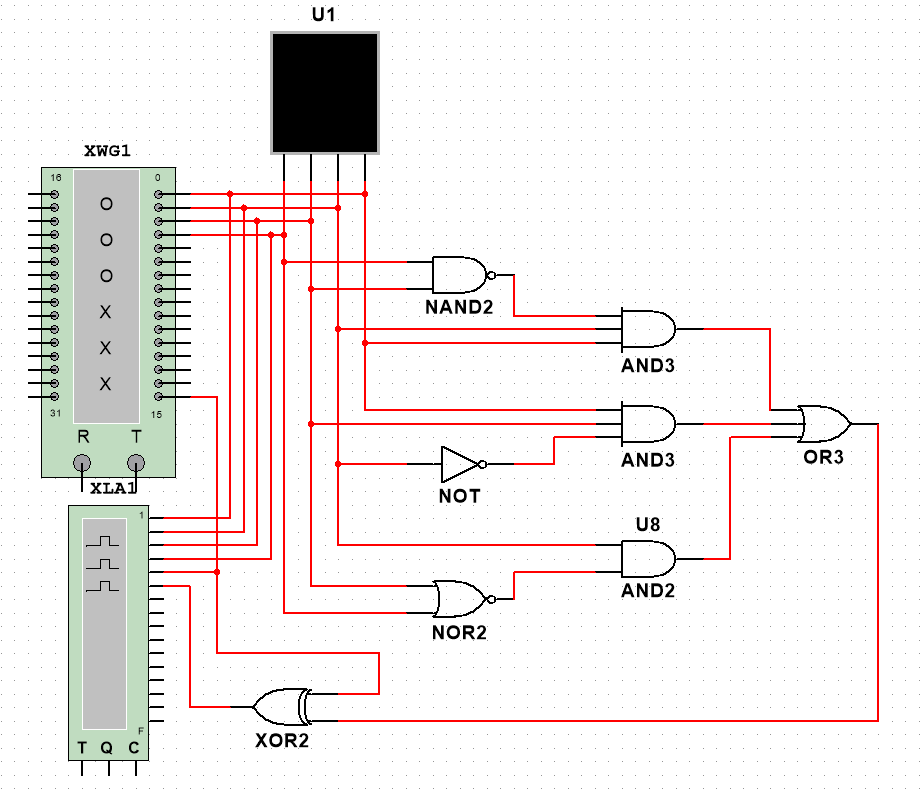
\includegraphics[width=1\textwidth]{images/1b_schema_2.PNG}
    \caption{Układ testowy}
    \label{rys:1b_test_circuit}
\end{figure}
\begin{figure}[H]
    \centering
    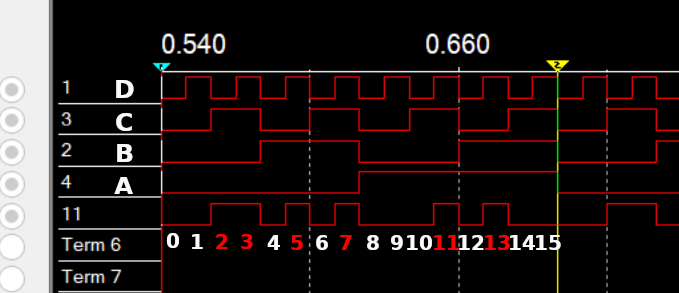
\includegraphics[width=1\textwidth]{images/1b_result.PNG}
    \caption{Wskazania analizatora}
    \label{rys:1b_test_results}
\end{figure}
Ze wskazań analizatora można stwierdzić że dla każdego możliwego słowa bitowego otrzymano poprawną wartość.
Układ wygenerował stan wysoki dla słów odpowiadającym 2,3,5,7,11,13.
\section{Wnioski}
\begin{enumerate}
    \item Układ jest prosty do zaimplementowania ponieważ polega na bezpośrednim mapowaniu danych wejściowych do oczekiwanego
    wyjścia ale przez to nie jest to rozwiązanie które można by skalować dla dłuższych słów bitowych.
    \item Sprzętowe generowanie liczb pierwszych może wspomóc oprogramowanie wykonujące testy pierwszości
    poprzez szybkie sprawdzenie małych liczb pierwszych.
    \item W celu przeskalowania układu do praktycznych zastosowań można użyć układów sprzętowego tablicowania wartości 
\end{enumerate}
\section{Podsumowanie}
\begin{enumerate}
    \item Funkcja logiczna została przekształcona do postaci pozwalającej na użycie jak najmniejszej ilości bramek.
    \item Układ pozwala identyfikować słowa binarne reprezentujące liczby pierwsze.
    \item Przetestowano poprawność układu stosując analizator stanów logicznych i generator słów losowych.
\end{enumerate}
\end{document}